%----------------------------------------------------------------------------------------
%
% A LaTeX-template for 1DV510. Modified and translated by Björn Lindenberg at LNU.
% Based on an original master thesis template created by Marcus Wilhelmsson at LNU.
%
%----------------------------------------------------------------------------------------

% Settings and document configuration

\documentclass[a4paper,12pt]{article} 
\usepackage[T1]{fontenc} 
\usepackage{times}

\usepackage[british]{babel} 
\usepackage[utf8]{inputenc}  
\usepackage{wallpaper} 
\usepackage[absolute]{textpos} 
\usepackage[top=2cm, bottom=2.5cm, left=3cm, right=3cm]{geometry} 
\usepackage[parfill]{parskip} 
\usepackage{csquotes} 
\usepackage{float} 
\usepackage{lipsum} % Used for dummy text. Can be removed.
\usepackage[backend=biber, style=ieee]{biblatex}
\addbibresource{ref.bib}
% Fontsizes for section headings.
\usepackage{sectsty} 
\sectionfont{\fontsize{14}{15}\selectfont}
\subsectionfont{\fontsize{12}{15}\selectfont}
\subsubsectionfont{\fontsize{12}{15}\selectfont}

%----------------------------------------------------------------------------------------
%	This part is used for the text box on the title page
%----------------------------------------------------------------------------------------
\newsavebox{\mybox}
\newlength{\mydepth}
\newlength{\myheight}

\newenvironment{sidebar}%
{\begin{lrbox}{\mybox}\begin{minipage}{\textwidth}}%
		{\end{minipage}\end{lrbox}%
	\settodepth{\mydepth}{\usebox{\mybox}}%
	\settoheight{\myheight}{\usebox{\mybox}}%
	\addtolength{\myheight}{\mydepth}%
	\noindent\makebox[0pt]{\hspace{-20pt}\rule[-\mydepth]{1pt}{\myheight}}%
	\usebox{\mybox}}

%----------------------------------------------------------------------------------------
%	Title
%----------------------------------------------------------------------------------------
\newcommand\BackgroundPic{
	\put(-2,-3){
		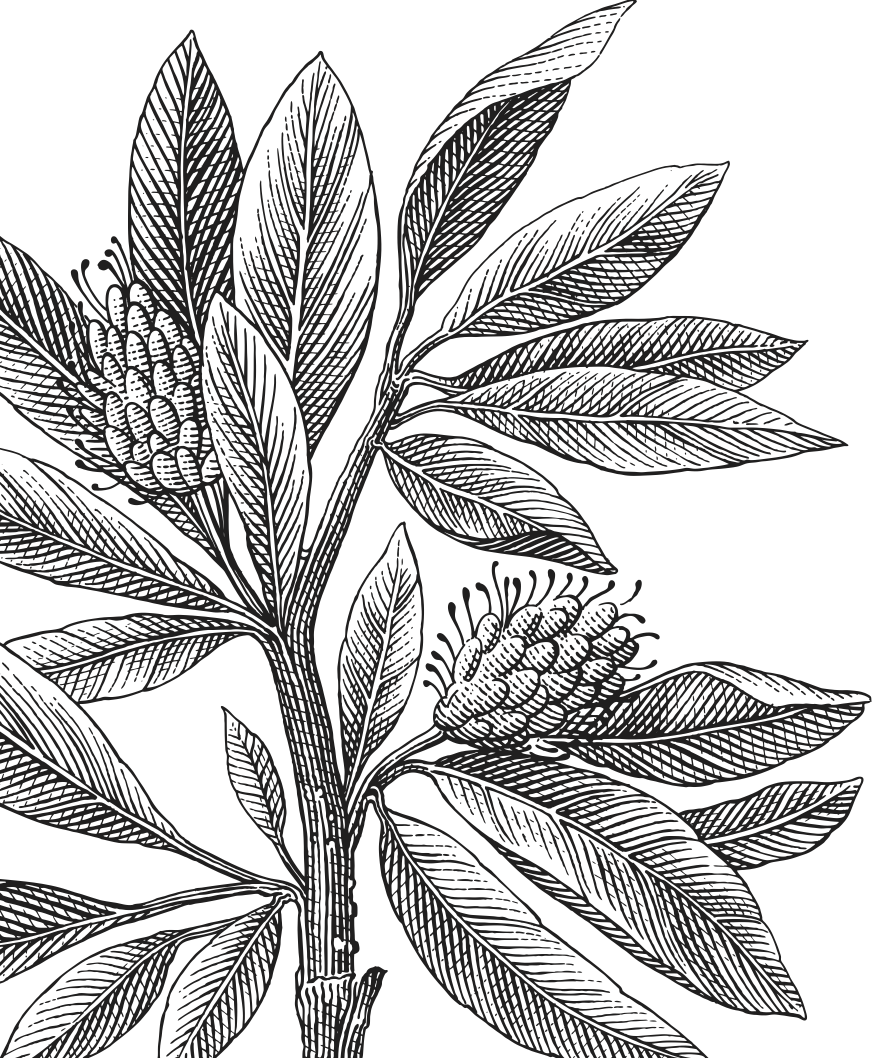
\includegraphics[keepaspectratio,scale=0.3]{img/lnu_etch.png} % Background image
	}
}
\newcommand\BackgroundPicLogo{
	\put(30,740){
		
\includegraphics[keepaspectratio,scale=0.10]{img/logo.png} % LNU logo
	}
}

\title{
	\vspace{-8cm}
	\begin{sidebar}
		\vspace{10cm}
		\normalfont \normalsize
		\huge Linnaeus University\\ % Main title
		\vspace{-1.3cm}
	\end{sidebar}
	\vspace{3cm}
	\begin{flushleft}
		\huge 2DV513 - Database Theory \\ Assignment 3%Subtitle
	\end{flushleft}
	\null
	\vfill
	\begin{textblock}{5}(10,13)
		\begin{flushright}
			\begin{minipage}{\textwidth}
				\begin{flushleft} \large
					\emph{Students}\\ Albert \textsc{T\'ellez}\\  
					Heysem \textsc{Askan} \\
					% Author
					 % Area
					\emph{Student ID}\\ at222vk, ab224hv %the id
				\end{flushleft}
			\end{minipage}
		\end{flushright}
	\end{textblock}
}

\date{} % Empty date command. Use \today inside for today's date.
\author{} % Normally one would use this to define authors. However in this case the title command takes care of everything, so we leave the field empty to get rid of warnings. 

\begin{document}
	

	
	
	
	\newgeometry{left=5cm}
	\AddToShipoutPicture*{\BackgroundPic} % Adds the background image to the title page
	\AddToShipoutPicture*{\BackgroundPicLogo} % Adds the logo to the title page
	\maketitle % Prints the title
	\thispagestyle{empty}
	\restoregeometry
	\clearpage


\tableofcontents

\clearpage

\section{Idea}
For our project we came up with a multi-functional music searching and sorting program. Our program solves a the difficulties faced by music lovers who would like to keep track of songs they like and search for them based on the lyrics, artist name and even the album name. 

Thanks to this program they could add, remove and search their favourite songs, artists and albums. The target audience for this program are the people who enjoy being able to store their music and classify it. A note-worthy function is the ability to search the song by the lyrics where the user will manage to find the song name when they happen to have an earworm. If multiple users make use of the program, with a large enough database other users would be able to search for songs even if they have not added them personally.

If they remember even a word from the lyrics, they can initiate a search using that word and find the song they are looking for as well as details about the singer that sang it and details about the album the song belongs to.
\clearpage

\section{Logical Model}
\begin{figure}[h]
	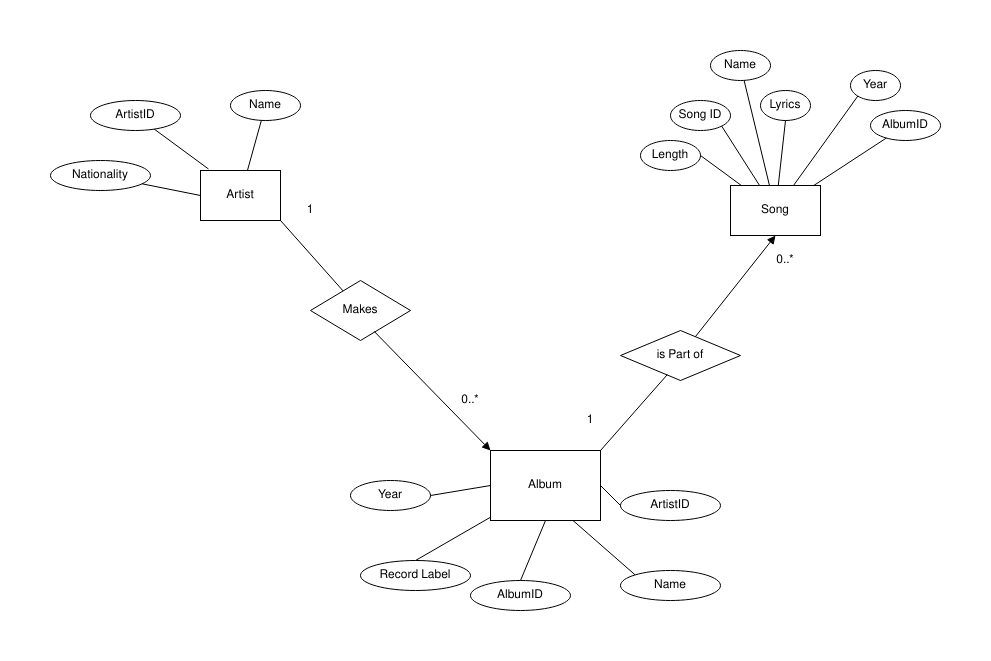
\includegraphics[width=\linewidth]{img/DB3Diagram.png}
	\caption{ER diagram of the database}
	\label{erdiag}
\end{figure}

Figure \ref{erdiag} shows the ER diagram that was used in the database. Beginning from the top left the Artist entity set can be found with an ID, so that each row could be easily identifiable. Nationalities and names were fields that would be quite reasonable information to store about an artist.

In the middle, the Album entity set can be found. This has some reasonable fields such as the year, the record label and the name of the album. The ArtistID field will allow to relate this entity set to the Artist entity set. 

Finally in the top right there is a Song entity set  that contains other reasonable fields, notably an album ID to relate it to the album, and a song ID that makes each row easily identifiable.
The Song entity set and the Album entity set both have a "year" property, which might seem slightly redundant. This is justified due to the fact that an album might have been released in a certain year, yet the song belonging to that album might have been released several years after the album

As can be seen in the diagram the database has some sort of inverse tree structure, in the sense that one artist can have many albums, and each individual album can have many songs belonging to it.


\clearpage
\section{Design in SQL}
The ER diagram translated into the following structure in SQL.

There are three tables created in the SQL database. The first table that was created is the Artists table, since it has no other requirements. Following that the Albums table is created since it depends on the Artists table, and finally the Songs table which depends on the Albums table.

The Artists table will contain all the artists in the database. There are three attributes. Firstly an ArtistID that is the unique key, and auto increments on every addition. Secondly a country that will be represented with two digits according to ISO 3166-1 alpha-2. This field will be a varchar in the database. Another field will be the name of the artist, which will also be a varchar with a length of 50, since it was deemed unnecessary to have longer strings for the artist names.



The next table created was called “Albums” which will contain all the albums in our database. Each of them have to be belong to an artist in the database. The Albums table has 5 attributes: AlbumID, ArtistID, Year, Name and Record Label. AlbumID attribute is a unique individual ID number given to each album in the database. It is the primary key auto-incrementing attribute for the Albums table. The ArtistID attribute is the ID number of the artist that created the album, set as a foreign key. The Year attribute is the year the album was initially released. The Name attribute is the name of the album. Record Label attribute is the name of the record label that marketed the album.
All the attributes except the IDs or the year, which are integers, are varchars with the length of 50.

Finally the last table created was the “Songs” table which will contain all the songs in our database. Each song has to be released in  an album created by the artist that made the song. In the case of "single" releases, the album will have the same name as the release of the song.


The Songs table has 6 attributes: SongID, AlbumID, Year, Name, Length, Lyrics.
SongID attribute is a unique individual id number given to each song in the database, it is the primary key auto-incrementing  attribute for the Songs table. AlbumID attribute is the id number of the album that the song belongs to, configured as a foreign key. Year attribute is the year the song was released. The Name attribute is the name of the song. The Length attribute is the length of the song in seconds. Finally the Lyrics attribute contains the lyrics of the song.


All the ID attributes whether own or foreign are configured to be integers. Years and length will also be configured as integers. The rest of the variables will be configured as varchars of length 50 except the Lyrics attribute, which will be configured as a text field that can store much longer strings, as would be needed for the lyrics of a song.

\clearpage


\section{SQL Queries}

Our program consists of a number of different SQL queries, but only a few were the necessary queries needed for the assignment.

We did not believe it was necessary to include the literal SQL queries in the report, therefore it will be stated that all the SQL queries can be found inside the EditDB class in the source code.

Two of our queries that implement data from more than one table are the search song by name and the search song by lyrics functionalities.


\begin{enumerate} 
	\item The first query, implementing the search by song feature, will perform an inner join on all the tables, since in order to get the name of the artist that released a specific song, a link between the albums and the artists is required. This was done by linking the unique IDs that appear in each of the tables together. After this the name column is switched into lowercase, then compared with the user inputs, which are also switched to lowercase. Wildcards are added to the query so matches containing that name are also returned.
	
	\item The second query respectively is used to perform a case insensitive search on the lyrics of a song. This function will also perform an inner join in the three tables of the database based on the ID. Once again, the column containing the lyrics will be turned into lowercase, afterwards the input lyrics of the will be inserted into lowercase, adding wildcards to ensure the highest possibility of a match.

	\item Another query that uses SQL join to a lesser extent is the query that will order songs by length, and similar. In this case the database will join only the songs and the albums table, performing an inner join. This is used to show the name of the song as well as the album that specific song belongs to. Then, the ASC or DESC keywords will be used in the query to represent the order the songs should be displayed, based on the song length.
	
	\item The next query included can count all the songs that each individual artist has. The query will output a table with two columns. One of the columns will have the name of the artist, and the other column will have the amount of songs that artist has. As previously mentioned, all three tables need to be joined for this to work, due to the design of the database. In this case, a right outer join is being used. The reasoning for this being used is that in the case an artist does not have albums or songs related to them, they will still be added to the result of the query. The group keyword is included in order to group the output table by the name of the artist, ensuring that they will appear only once. Utilising the keyword count on the Songs.Name column can allow us to count the amount of songs per artist. This query will print all the artists in the database, which might lead to a long or unstable output, therefore, the query below would be recommended.
	
	\item Finally another query where grouping was implemented would be on the query that allows the user to count the songs of a specific artist. The implementation for this query is essentially the same as for the query above, except in this scenario a "having" clause is implemented in order to match with a specific artist ID.
\end{enumerate}

\section{Supplemental video}

We created a video showcasing some of the functions that we implemented in the database. The video can be found in the following link:

\url{https://www.youtube.com/watch?v=83ckmYkIA00}

In the submission there will also be a small database dump so that the functionality can be tried. It is to note that one small setback of adding songs is that due to the nature of command-line interfaces, pasting any input that contains a line break will trigger the "enter" function of the input.

\end{document}

